\section{Dyskretne ilorazy rozmaitości}

\subsection{Klejenie rozmaitości wzdłuż brzegu}

\phantomsection\label{otoczenie kolnierzowe definicja}
\begin{theorem}[otoczenie kołnierzowe] Niech $M$ będzie gładką $n$-rozmaitościa, a $B$ niech będzie kompotentą brzegu $\partial M$. Wtedy istnieje dyfeomorficzne (dyfeomorfizm na obraz) włożenie
  $$K:B\times[0, 1)\to M$$
  na otwarte otoczenie $U$ komponenty $B$ w $M$ takie, że $K(x, 0)=x$ dla $x\in B$.

  \important{Otoczenie kołnierzowe} to otwarte otoczenie $U$ brzegu $\partial M$ na $M$, wraz z dyfeomorfizmem $F:[0,1)\times\partial M\to U$ takie, że $F(0,x)=x$.
\end{theorem}

\begin{proof}Dowód za kilka wykładów przy pomocy potoków wektorowych (\hyperref[dowod otoczenia kolnierzowego]{Rozdział 5.4}).

  \begin{illustration}
    \filldraw[orange!25] (6.5, 0) arc (0:360: 0.5cm and 1cm);
    \filldraw[orange!25] (6, 1)--(7, 1)--(7, -1)--(6, -1);
    \draw[rounded corners=35pt](7,-1)--(4.2,-1)--(2,-2)--(0,0) -- (2,2)--(4.2,1)--(7,1);
    \draw (1.5,0.2) arc (175:315:1cm and 0.5cm);
    \draw (3,-0.28) arc (-30:180:0.7cm and 0.3cm);
    \filldraw[color=black, fill=white] (7.5,0) arc (0:360:0.5cm and 1cm);
    \node (a) at (20:2.5) {$M$};
    %\node (a) at (-12:7.5) {$\partial M=N$};
    \node at (7.8, 0) {$B$};

    \node at (6, 0) {$\color{orange}U$};
  \end{illustration}
\end{proof}

Jeśli $M_1,B_1$ oraz $M_2,B_2$ są jak wyżej oraz istnieje dyfeomorfizm
$$f:B_1\to B_2$$
to możemy zdefiniować relację równoważności
$$B_1\ni x\sim f(x)\in B_2$$
oraz stworzyć rozmaitość:
$$M_1\cup_fM_2=M_1\sqcup M_2/\sim.$$

\textbf{Struktura} na $M_1\cup_fM_2$ jest częściowo odziedziczona po $M_1$ i $M_2$. Dodatkowo sklejamy zbiory $U_i$ utożsamiając je z produktami $B_i\times[0,1)$ za pomocą $B_i$:
$$K_i:B_i\otimes [0,1)\to M_i$$

\begin{center}\scalebox{0.7}{
  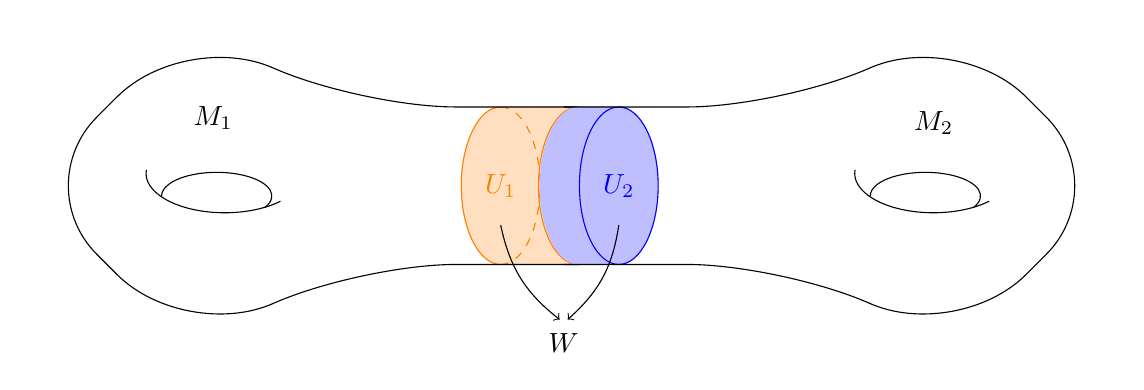
\begin{tikzpicture}
    \filldraw[orange!25] (6.5, 0) arc (0:360: 0.5cm and 1cm);
    \filldraw[orange!25] (6, 1)--(7, 1)--(7, -1)--(6, -1);
    \draw[orange] (6, 1) arc (90:270:0.5cm and 1cm);
    \draw[orange, dashed] (6, 1) arc (90:-90:0.5cm and 1cm);
    \draw[orange] (6.98, 1) arc (90:270:0.5cm and 1cm);
    \draw[rounded corners=35pt](7,-1)--(4.2,-1)--(2,-2)--(0,0) -- (2,2)--(4.2,1)--(7,1);
    \draw (1.5,0.2) arc (175:315:1cm and 0.5cm);
    \draw (3,-0.28) arc (-30:180:0.7cm and 0.3cm);
    \filldraw[blue!25] (7.5,0) arc (0:360:0.5cm and 1cm);
    \node (a) at (20:2.5) {$M_1$};
    %\node (a) at (-12:7.5) {$\partial M=N$};
    %\node at (7.8, 0) {$B_1$};

    \node at (6, 0) {$\color{orange}U_1$};

    \filldraw[blue!25] (8,0) arc (0:360:0.5cm and 1cm);
    \filldraw[blue!25] (7.5, 1)--(7, 1)--(7, -1)--(7.5, -1);
    %\draw[blue, thick] (7.01, 1) arc (90:270:0.5cm and 1cm);
    \draw[blue] (8,0) arc (0:360:0.5cm and 1cm);
    \node at (7.5, 0) {$\color{blue}U_2$};

    \draw[rounded corners=35pt, rotate around={180:(6.9, 0)}](7,-1)--(4.2,-1)--(2,-2)--(0,0) -- (2,2)--(4.2,1)--(7,1);

    \draw (10.5,0.2) arc (175:315:1cm and 0.5cm);
    \draw (12,-0.28) arc (-30:180:0.7cm and 0.3cm);
    \node at (11.5, 0.8) {$M_2$};

    \node at (6.8, -2) {$W$};

    \path[->] (6, -0.5) edge [bend right=20] (6.75, -1.7);
    \path[->] (7.5, -0.5) edge [bend left=20] (6.85, -1.7);
  \end{tikzpicture}
}\end{center}

Na $M_1\cup_fM_2$ istnieją trzy rodzaje map:
\begin{enumerate}
  \item dla dowolnej mapy $(U,\phi)$ na $M_1$ rozważamy jej obcięcie do $U\setminus B_1$
  \item dla dowolnej mapy $(V,\psi)$ na $M_2$ rozważamy jej obcięcie do $V\setminus B_2$
  \item dla dowolnej mapy $(W,\xi)$ na $B_1$ i $\xi:W\to\overline{W}\subseteq\R^{n-1}$ rozważamy zbiór 
    $$[W\times[0,1)]\cup_{f\restriction W}[f(W)\times[0,1)]=\hat{W}\subseteq M_1\cup_fM_2$$
    z mapą 
    $$\hat{\xi}:\hat{W}\to\overline{\hat{W}}\subseteq\R^n$$
    $$\hat{\xi}(x, t)=\begin{cases}(\xi(x),-t)&(x,t)\in U_1\\(\xi(f^{-1}(x)), t)&(x,t)\in U_2\end{cases}$$
    Mamy $\hat{\xi}(x, 0)=\hat{\xi}(f(x), 0)$, więc $\hat{x}$ jest dobrze zdefiniowane w punktach sklejenia. 
    $$\overline{\hat{W}}=\overline{W}\times(-1,1)\subseteq\R^n\times (-1,1)\subseteq\R^{n+1}$$
    zaś $\hat{\xi}:\hat{W}\to\overline{\hat{W}}$ jest homeomorfizmem.
\end{enumerate}

Sprawdzenie gładkiej zgodności map z podpunktów 1, 2 i 3 zostanie pominięte.

Rozmaitość $M_1\cup_fM_2$ wydaje się zależeć jednocześnie od wyboru $f$ oraz otoczeń kołnierzowych $K_i$ komponent brzegów $B_i$. W rzeczywistości jednak, $M_1\cup_fM_2$ jest takie same z dokładnością do dyfeomorfizmu dla dowolnych wyborów $K_i$:

\begin{fact}$ $\newline
  \begin{enumerate}
    \item Jeśli $K_1,K_1'$ są podobnie położone w $M_1$, tzn. istnieje $h:M_1\to M_1$ dyfeomorfizm taki, że 
      $$K_1'\restriction B_1\times[0,1\frac12)=h\circ K_1\restriction B_1\times[0,\frac12),$$ 
      to wtedy 
      $$M_1\cup_{f,K_1,K_2}M_2\cong M_1\cup_{f,K_1',K_2}M_2.$$
      Analogicznie gdy weźmiemy $K_2,K_2'$. [dowód: ćwicznia] 
    \item Każde dwa otoczenia kołnierzowe komponenty $B_1$ brzegu $\partial M$ są podobnie położone. [dowód trudny] 
    \item Ustalmy otoczenia kołnierzowe $K_1,K_2$. Jeśli $f_0,f_1:B_1\to B_2$ są izotopijnymi dyfeomorfizmami, tzn. istnieje gładkie $F:[0,1]\times B_1\to B_2$ takie, że $F(0)=f_0$ a $F(1)=f_1$, wtedy 
      $$M_1\cup_{f_0,K_1,K_2}M_2\cong M_1\cup_{f_1,K_1,K_2}M_2.$$
      [dowód łatwy]
  \end{enumerate}
\end{fact}

\subsection{Suma spójna rozmaitości}

Niech $M_1,M_2$ będą rozmaitościami wymiaru $n$. Weźmy $D_i\subseteq M_i$, czyli kule $n$-wymiarowe zawarte w otoczeniach mapowych. Oznaczmy $B_i=\partial D_i\cong S^{n-1}$ jako komponenty brzegu rozmaitości $M_i\setminus Int(D_i)$. Niech
$$f:B_1\to B_2$$
będzie dyfeomorfizmem. Oznaczamy wówczas
$$[M_1\setminus Int(D_1)]\cup_f[M_2\setminus Int(D_2)]=\color{blue}M_1\#M_2$$
jako \important{sumę spójną} rozmaitości $M_1$ i $M_2$.

\begin{illustration}
  \draw[rounded corners=35pt, rotate around={180:(4, 0)}](6,-1)--(4.2,-1)--(2,-2)--(0,0) -- (2,2)--(4.2,1)--(6,1);
  \draw (3,0.2) arc (175:315:1cm and 0.5cm);
  \draw (4.5,-0.28) arc (-30:180:0.7cm and 0.3cm);
  \draw (2.5,0) arc (0:360:0.5cm and 1cm);
  \node (a) at (4.5, 0.6) {$M_1$};
  \filldraw[color=blue, fill=blue!30] (6, 0.2) circle (0.6);

  \draw (10, 0) ellipse (2cm and 1.3cm);
  \filldraw[color=blue, fill=blue!30, rotate around={30:(8.9, 0.5)}] (8.9, 0.5) ellipse (0.6 and 0.4);
  \draw (9.5, 0) arc (160:20:0.8 and 0.4);
  \draw (9.3, 0.2) arc (200:340:1 and 0.6);
  \node at (10.5, 0.9) {$M_2$};
  \node at (6, 1) {$D_1$};
  \node at (8.9, 1.2) {$D_2$};
\end{illustration}

\begin{illustration}
  \draw[rounded corners=35pt, rotate around={180:(4, 0)}](6,-1)--(4.2,-1)--(2,-2)--(0,0) -- (2,2)--(4.2,1)--(6,1);
  \draw (3,0.2) arc (175:315:1cm and 0.5cm);
  \draw (4.5,-0.28) arc (-30:180:0.7cm and 0.3cm);
  \draw (2.5,0) arc (0:360:0.5cm and 1cm);
  \node (a) at (4.5, 0.6) {$M_1$};
  %\filldraw[color=blue, fill=blue!30] (7, 0) circle (0.6);

  \draw (9, 0) ellipse (2cm and 1.3cm);
  %\filldraw[color=blue, fill=blue!30, rotate around={30:(8.9, 0.5)}] (8.9, 0.5) ellipse (0.6 and 0.4);
  \draw (8.5, 0) arc (160:20:0.8 and 0.4);
  \draw (8.3, 0.2) arc (200:340:1 and 0.6);
  \node at (10, 0.9) {$M_2$};
  %\node at (6, 1) {$D_1$};
  %\node at (8.9, 1.2) {$D_2$};
  \filldraw[color=blue, fill=blue!25] (7.3, 0) ellipse (0.4 and 0.7);
\end{illustration}

\begin{illustration}
  \draw[rounded corners=35pt, rotate around={180:(4, 0)}](6,-1)--(4.2,-1)--(2,-2)--(0,0) -- (2,2)--(4.2,1)--(6,1);
  \draw (3,0.2) arc (175:315:1cm and 0.5cm);
  \draw (4.5,-0.28) arc (-30:180:0.7cm and 0.3cm);
  \draw (2.5,0) arc (0:360:0.5cm and 1cm);
  \node (a) at (4.5, 0.6) {$M_1$};
  %\filldraw[color=blue, fill=blue!30] (7, 0) circle (0.6);

  \draw (9, 0) ellipse (2cm and 1.3cm);
  %\filldraw[color=blue, fill=blue!30, rotate around={30:(8.9, 0.5)}] (8.9, 0.5) ellipse (0.6 and 0.4);
  \draw (8.5, 0) arc (160:20:0.8 and 0.4);
  \draw (8.3, 0.2) arc (200:340:1 and 0.6);
  \node at (10, 0.9) {$M_2$};
  %\node at (6, 1) {$D_1$};
  %\node at (8.9, 1.2) {$D_2$};
  \filldraw[white] (7.3, 0) ellipse (0.5 and 1);
  \draw (7.08, 0.9) arc(250:285:0.8);

  \draw (7.08, -0.9) arc(110:75:0.8);
  \draw[dashed] (7.3, 0) ellipse (0.3 and 0.85);
\end{illustration}

\begin{remark}$ $\newline
  \begin{enumerate}
    \item Jeśli $M_i$ jest rozmaitością spójną, to $M_i\setminus Int(D_i)$, z dokładnością do dyfeomorfizmu, nie zależy od wyboru dysku $D_i$.
    \item Istnieją dokładnie $2$ klasy izotopii dyfeomorfizmów $f:S^{n-1}\to S^{n-1}$: te zachowujące orientację oraz te, które orientacji nie zachowują.
    \item Są co najwyżej dwie rozmaitości będące sumą spójną $M_1\#M_2$. W przypadku rozmaitości zorientowanych, jedna z nich jest preferowana.
  \end{enumerate}
\end{remark}

\textbf{Klasyfikacja zamkniętych powierzchni spójnych} (czyli zwarte $2$-wymiarowe rozmaitości bez brzegu):
\begin{enumerate}
  \item Powierzchnie orientowalne: $S^2, T^2, T^2\#T^2,T^2\#T^2\#T^2,...$
  \item Powierzchnie nieorientowalne $\R P^2=S^2/\Z_2,\R P^2\#\R P^2,...$
\end{enumerate}
Powierzchnie z powyższej listy są parami niedyfeomorficzne. Każda zamknięta powierzchnia jest dyfeomorficzna z jedną z tej listy.

\textbf{$3$-rozmaitości:}\marginpar{Poniżej bardzo luźne opisy z wikipedii. Dokładniejsze opisy lepiej jest doczytać w literaturze.}
\begin{itemize}
  \item[\PHtunny] \acc[b]{Dehn surgery:} niech $M$ będzie $3$-wymiarową rozmaitością $M$ z kolekcją węzłów (podrozmaitości $S^n$ dyfeomorficznych do skończonej rozłącznej sumy $S^j$) $L=L_1\cup...\cup L_k$. Rozmaitość $M$ wywiercona wzdłuż tubowego otoczeniem $L$ posiada $k$-wiele komponentów brzegu $T_1\cup...\cup T_k$. Chirurgia Dehna polega na wywierceniu z $M$ tubowego otoczenia $L$ wraz ze sklejeniem każdej z komponent brzegu $T_1\cup...\cup T_k$ w jeden torus [to jest Dehn filling i jest wiele sposobów na wytworzenie go].
  \item[\PHtunny] \acc[d]{Rozkłady Heegaarda} [Heegaard's splittings] na zorientowanej $3$-rozmaitości z brzegiem $M$ polega na na podzieleniu jej na dwa handlebody [fidget spinnery; $3$-rozmaitości oriengowalne z brzegiem zawierające parami rozłączne włożone $2$-dyski takie, że rozmaitość wzdłuż nich przecięta jest $S^3$].
    \begin{illustration}
      \filldraw[color=black, fill=white] (0, 0) ellipse (1.8 and 1.5);
      \filldraw[color=black, fill=white] (2.5, 0) ellipse (1.8 and 1.5);
      \filldraw[white] (1.25, 0) ellipse (0.8 and 1.2);
      \filldraw[color=black, fill=white] (1.25, -2.2) ellipse (1.8 and 1.5);
      \filldraw[white] (1.25, -1.5) ellipse (1.9 and 1);
      \draw (0, 0) ellipse (0.6 and 0.5);
      \draw (2.5, 0) ellipse (0.6 and 0.5);
      \draw (1.25, -2.2) ellipse (0.6 and 0.5);
      \draw (1.1, 1.2) arc (240:300:0.3);
      \draw (-0.7, -1.38) arc (70:-30:0.35);
      \draw (3.2, -1.38) arc (110:210:0.35);
      \node at (4.8, -2) {\scriptsize genus $3$ handlebody};
      \path [->] (4.8, -2.3) edge [bend left=40] (3.2, -3);
    \end{illustration}
\end{itemize}

\subsection{Działanie grupy dyfeomorfizmów}

\begin{definition}[grupa dyfeomorfizmów] Grupa $G$ dyfeomorfizmów $M$ to zbiór dyfeomorfizmów $g:M\to M$ zamknięty na składanie i branie odwrotności. Mówimy wtedy, że $G$ działa na $M$ przez dyfeomorfizmy.
\end{definition}

\begin{definition}[orbita] \important{Orbitą} punktu $x\in M$ względem działania $G$ na $M$ nazywamy zbiór
  $$\color{blue}G(x)=\{g(x)\;:\;g\in G\}$$
\end{definition}

\begin{remark} Orbity $G(x)$ i $G(y)$ są albo rozłączne, albo pokrywają się.
\end{remark}

Rodzina wszystkich orbit stanowi \acc[b]{rozbicie} rozmaitości $M$ na podzbiory.

\begin{definition}[przestrzeń ilorazowa działania $G$ na $M$] \important{Przestrzeń ilorazowa} działania $G$ na $M$ to przestrzeń, której punktami są orbity $G(x)$:
  $$\color{blue}M/G=\{G(x)\;:\;x\in M\}$$
  zaś topologia jest ilorazowa, tzn. \acc[i]{zbiór orbit jest otwarty} w $M/G$ $\iff$ suma tych orbit stanowi otwarty podzbiór w $M$.
\end{definition}

Jeśli $U\subseteq M$ jest otwartym podzbiorem, to 
$$\color{blue}G(U)/G=\{G(x)\;:\;x\in U\}$$
jest otwarty w $M/G$ i każdy zbiór otwarty w $M/G$ jest takiej postaci. Kiedy $\set{B}$ jest bazą topologii w $M$, to rodzina
$$\{G(U)/G\;:\;U\in\set{B}\}$$
jest \acc[b]{bazą topologii} w $M/G$. Z tego powodu $M/G$ \textbf{zawsze posiada przeliczalną bazę}.

\begin{definition}[działanie nakrywające] Lokalną euklidesowość $M/G$ zapewnia warunek na \important{działanie nakrywające}:
  $$(\forall\;p\in M)(\exists\;p\in U\overset{otw.}{\subseteq}M)(\forall\;g_1,g_2\in G)\;g_1(U)\cap g_2(U)=\emptyset.$$
  Przy takim działaniu $G$ na $M$ podzbiór $G(U)/G$ jest otoczeniem $G(p)$ homeomorficzny z $U$. Oznacza to lokalną euklidesowość $M/G$.
\end{definition}

\begin{fact}
  Jeśli działanie grupy$G$ przez homeomorfizmy na rozmaitości $M$ jest nakrywające, to iloraz $M/G$ jest lokalnie euklidesowy dla wymiaru $n=dim(M)$.
\end{fact}

\begin{example}
\item Działanie grupy $\Z$ na $\R^2\setminus\{(0, 0)\}$ przez potęgi przekształcenia liniowego zadanego macierzą
  $$A=\begin{pmatrix}2&0\\0&\frac{1}{2}\end{pmatrix}$$
  jest nakrywające. W takim razie iloraz $(\R^2\setminus\{(0,0)\})/\langle A\rangle$ jest lokalnie euklidesowy wymiaru $2$. Jednak iloraz ten nie jest przestrzenią Hausdorffa, bo dla punktów na osobnych osiach $p$ i $q$ zbiory otwarte:
  
  \begin{illustration}
    \draw[<-] (0, 4.5)--(0, -4.5);
    \draw[->] (-4.5, 0)--(4.5, 0);
    \filldraw (0, 3) circle (1.5pt) node [right] {$q$};
    \filldraw (3, 0) circle (1.5pt) node [below] {$p$};

    \draw[blue, thick] (-0.5, 2.5) rectangle (0.5, 3.5);
    \node at (-0.3, 3.8) {$\color{blue}V$};
    \draw[blue, thick] (-1, 1.25) rectangle (1, 1.75);
    \draw[blue, thick] (-2, 0.625) rectangle (2, 0.875);
    \draw[blue, thick] (-4, 0.3125) rectangle (4, 0.4375);

    \draw[orange, thick] (2.5, -0.5) rectangle (3.5, 0.5);
    \node at (3.3, 0.8) {$\color{orange}U$};
    \draw[orange, thick] (1.25, -1) rectangle (1.75, 1);
    \draw[orange, thick] (0.625, -2) rectangle (0.875, 2);
    \draw[orange, thick] (0.3125, -4) rectangle (0.4375, 4);
  \end{illustration}
  nigdy nie mogą być rozłączne. Stąd rozmaitość ilorazowa $M/G$ nie może być nigdy rozmaitością różniczkowalną.
\end{example}

\begin{definition}[działanie wolne, właściwie nieciągłe]
  Działanie $G$ na $M$ przez dyfeomorfizm jest:
  \begin{enumerate}
    \item \important{wolne}, gdy dla każdego $g\in G\setminus\{id\}$ i dla każdego $x\in M$ $g(x)\neq x$
    \item \important{właściwie nieciągłe} [properly discontinuous], gdy dla każdego zwartego $K\subseteq M$ zbiór $\{g\in G\;:\;g(K)\cap K\neq \emptyset\}$ jest skończony.
  \end{enumerate}
\end{definition}

\begin{definition}[stabilizator]
  Dla $x\in M$ \acc[b]{stabilizator} (nadgrupa stabilizująca) punktu $x$ względem $G$ to
  $$\color{blue} Stab(x):=\{g\in G\;:\;g(x)=x\}$$
  jest automatycznie podgrupą $G$.
\end{definition}

\begin{fact}
  Działanie $G$ jest wolne $\iff$ wszystkie stabilizatory $stab(x)$ są trywialne ($=\{id\}$).
\end{fact}

\begin{example}
  \item Działanie grupy $\Z_n$ na $\R^2$ zadane przez potęgi obrotu o kąt $\frac{2\pi}{n}$ nie jest wolne.
  \item Działanie $G$ jest wolne $\iff$ dla każdego $x\in M$ odwzorowanie $G\to G(x)$ zadane przez $g\mapsto g(x)$ jest bijekcją.
\end{example}

\begin{fact}$ $\newline
  \begin{enumerate}[leftmargin=*]
  \item Gdy działanie $G$ przez homeomorfizmy na przestrzeni topologicznej lokalnie zwartej $X$ jest właściwie nieciągłe, to każda orbita $G(x)$ jest dyskretnym podzbiorem w $X$ (tzn. każdy $x\in G(x)$ ma otwarte otocznie $U$ takie, że $U\cap G(x)=\{x\}$).
  \item Jeśli działanie $G$ na $X$ jest właściwie nieciągłe i wolne, to jest też nakrywające.

  \item Jeśli $G$ działa przez homeomorfizmy na przestrzeni lokalnie zwartej $X$ w sposób właściwie nieciągły, to iloraz $X/G$ jest przestrzenią Hausdorffa.
\end{enumerate}
\end{fact}

\begin{example}
  \item Działanie grupy $\Z$ na $S^1$ przez potęgi obrotu o kąt $\alpha$ niewspółmierny z $2\pi$ jest wolne, ale ma orbity gęste w $S^1$, a więc nie są one dyskretne. Zatem działanie nie jest ani właściwie nieciągłe, ani wolne. Iloraz $s^1/\Z$ jest wtedy przestrzenią z topologią trywialną, więc nie jest rozmaitością.
  \item Działanie $\Z$ na $\R^2\setminus\{(0,0)\}$ przez potęgi
    $$A=\begin{pmatrix}2&0\\0&\frac{1}{2}\end{pmatrix}$$
    nie może być właściwie nieciągłe. Można to zobaczyć bezpośrednio:
    \begin{illustration}
      \draw[<-] (0, 4)--(0, -3.8);
      \draw[->] (-4, 0)--(4, 0);
      \node at (0.6, 3.8) {$K$};
      \node at (1.4, 2) {$A(K)$};
      \node at (2.8, 1.1) {$A^2(K)$};
      \draw[thick] (-0.5, 3.5)--(0.8, 3.5)--(0.8, -0.5)--(0.5, -0.5)--(0.5, 3)--(-0.5, 3)--cycle;
      \draw[thick] (-1, 1.75)--(1.6, 1.75)--(1.6, -0.25)--(1, -0.25)--(1, 1.5)--(-1, 1.5)--cycle;
      \draw[thick] (-2, 0.875)--(3.2, 0.875)--(3.2, -0.125)--(2, -0.125)--(2, 0.75)--(-2, 0.75)--cycle;
    \end{illustration}
    dla każdego $n\geq 1$ mamy $A^n(K)\cap K\neq \emptyset$.

    Jednakże tak zadane działanie $\Z$ na $\R^2\setminus\{(0,0)\}$ jest wolne i ma dyskretne orbity. W takim razie warunek, by działanie było wolne i miało dyskretne orbity nie jest wystarczający do tego, by iloraz był rozmaitością. Nie musi być nawet przestrzenią Hausdorffa, jak pokazaliśmy wcześniej.
\end{example}

\begin{fact}
  Jeśli $G$ jest działaniem na $M^n$ przez dyfeomorfizmy w sposób wolny i właściwie nieciągły, to iloraz $M/G$ jest
  \begin{itemize}
    \item lokalnie euklidesowy $n$-wymiarowy
    \item Hausdorffa
    \item ma przeliczalną bazę
  \end{itemize}
  Zatem $M/G$ jest $n$-wymiarową rozmaitością topologiczną.
\end{fact}

\subsection{Gładki atlas na $M/G$}

Niech $U\subseteq M$ spełnia warunek:
\begin{center}
\phantomsection
\label{warunek_gladki_atlas}
  {\color{orange}(\PHcat)} $U$ jest zbiorem mapowym oraz dla każdych $g_1,g_2\in G$, $g_1\neq g_2\implies g_1(U)\cap g_2(U)=\emptyset$.
\end{center}

Zauważmy, że każdy $p\in M$ ma otoczenie $U$ spełniające \hyperref[warunek_gladki_atlas]{\color{orange}(\PHcat)}, a zatem każda orbita $G(p)\in M/G$ ma otoczenie postaci $G(U)/G$ ze zbiorem $U$ spełniającym \hyperref[warunek_gladki_atlas]{\color{orange}(\PHcat)}.  Dla takiego $U$ odwzorowanie
$$i_U:U\to G(U)/G$$
$$p\mapsto G(p)$$
jest homeomorfizmem. Niech teraz $\phi:I\to\overline{U}\subseteq \R^n$ będzie mapą z atlasu $\set{A}$. Wtedy
$$\phi_G:G(U)/G\to \overline{U}\subseteq\R^n$$
$$\phi_G=\phi\circ i_U^{-1}$$
jest obiecującym kandydatem na mapę dla $M/G$. Rozważmy rodzinę
$$\set{A}_G=\{(G(U)/G, \phi_G)\;:\;U \text{ spełnia \hyperref[warunek_gladki_atlas]{\color{orange}(\PHcat)} oraz }(U,\phi)\in\set{A}\}.$$
%Pokażemy, że wówczas
%\begin{itemize}
%  \item $\set{A}_G$ jest gładko zgodny, więc jest gładkim atlasem na $M/G$
%  \item odwzorowanie ilorazowe $q_G:M\to M/G$ zadane przez $q_G(x)=G(x)$ jest gładkie i jest lokalnym dyfeomorfizmem.
%\end{itemize}2
\begin{fact} Odwzorowanie ilorazowe $q_G:M\to M/G$ zadane przez
  $$q_G(x)=G(x)\in M/G$$
  jest gładkie i jest lokalnym dyfeomorfizmem.
\end{fact}

\begin{proof}$ $\newline
  \begin{illustration}
    \draw[<-] (0, 2)--(0, -2);
    \draw[->] (-2, 0)--(2, 0);
    \draw plot [smooth cycle] coordinates {(-1.5, 1) (-0.8, 1.5) (0.6, 1.3) (1.3, 0.8) (1.4, -0.5) (0.7, -1.7) (-0.4, -1.8) (-1.3, -0.3)};
    \path (3.5, -0.5) edge [bend left=10] (4, 1.5);
    \path (4, 1.5) edge [bend left=10] (7, 1.5);
    \path (7, 1.5) edge [bend right=10] (6.5, -0.5);
    \path (6.5, -0.5) edge [bend right=10] (3.5, -0.5);
    \draw plot [smooth cycle] coordinates {(4.3, 0.3) (4.5, 1) (5.3, 1.3) (6, 1) (5.4, 0.1) (4.7, -0.1) };
    \node at (6.2, 1.4) {$U$};
    \node at (4, 1.8) {$M$};
    \path[->] (4.3, 0.8) edge [bend right=20] node [above] {$\phi$} (1.3, 0.9);
    \node at (0.6, 1.5) {$\overline{U}$};
    \draw[rotate around={30:(5, -3)}] (5, -3) ellipse (1.8 and 1.5);
    \draw plot [smooth cycle] coordinates {(5, -2.8) (5.7, -2) (5.3, -1.8) (4.4, -2.1) (4, -2.5)};
    \path[->] (4.4, -2) edge [bend right=20] node [below] {$\phi_G=\phi\circ i_U^{-1}$} (1.4, -0.7);
    \path[->] (5.4, -0.1) edge [bend left=20] node [right] {$i_u=q_G\restriction U$} (5.4, -1.7);
    %\filldraw (6.4,-3.75) circle (1.5pt);
    %\filldraw (3.6, -2.25) circle (1.5pt);
    \path (6.4, -3.75) edge [bend left=15] (3.6, -2.25);
    \node at (6.5, -4) {$M/G$};
    \node at (6.3, -2.3) {$G(U)/G$};
    \node at (-2, -1) {$\R^n$};
  \end{illustration}
  Zakładamy, że $\set{A}_G$ tworzy gładki atlas [fakt \ref{gładki_atlas_na_ilorazie}]. Wtedy $q_G$ obcięte do mapowego $U$ musi spełniać \hyperref[warunek_gladki_atlas]{\color{orange}(\PHcat)}, więc jest bijekcją na otwary podzbiór w $M/G$. Ponadto
  $$\phi_G\circ q_G\circ\phi^{-1}=\phi\circ i_U^{-1}\circ i_U\phi^{-1}=id_{\overline{U}}$$
  czyli $q_G$ musi być funkcją gładką, bo inaczej $id_{\overline{U}}$ takie nie będzie. Stąd $q_G$ jest dyfeomorfizmem.
\end{proof}

\begin{fact}\label{gładki_atlas_na_ilorazie}
  $\set{A}_G$ jest gładko zgodny, więc jest gładkim atlasem na $M/G$.
\end{fact}

\begin{proof}
  Niech $(G(U)/G, \phi_G)$ oraz $(G(V)/G, \psi_G)$ będą mapami związanymi z $(U,\phi)$ i $(V,\psi)$ na zbiorach $U,V$ spełniającymi \hyperref[warunek_gladki_atlas]{\color{orange}(\PHcat)}. Rozważmy odwzorowanie przejścia
  $$\psi_G\circ\phi_G^{-1}:\phi_G(G(U)/G\cap G(V)/G)\to \psi_G(G(U)/G\cap G(V)/G)$$
  wiemy, że zachodzi
  $$\psi_G\circ\phi_G^{-1}=\psi\circ i_V^{-1}\circ[\phi\circ i_V^{-1}]^{-1}=\psi\circ i_V^{-1}\circ i_U\circ \phi^{-1}$$
  czyli wystarczy, żeby 
  $$i_V^{-1}i_U:U\cap i_U^{-1}(G(V)/G)\to V\cap i_V^{-1}(G(U)/G)$$
  było gładkie.
  \begin{illustration}
    \path (0, 0) edge [bend left=20] (1, 2);
    \path (1, 2) edge [bend left=10] (5, 2);
    \path (5, 2) edge [bend right=20] (4, 0);
    \path (4, 0) edge [bend right=10] (0, 0);

    %\draw plot [smooth cycle, round corners=5pt] coordinates {(1, 0.2) (0.6, 0.3)(1, 0.8) (1.3, 1.3) (1.1, 1.5) (1.5, 1.75) (1.8, 1.86) (3, 1.8) (4, 1.7) (4.3, 1.5) (4.1, 1.2) };
    %\draw plot [smooth cycle, round corners = 10pt] coordinates {(1.5, 0.3) (0.5, 0.7) (1.3, 1.3) (2.8, 1.7) (3.3, 1.8) (3.5, 1.7) (3.7, 1.3) (4.5, 0.7)};
    \filldraw[green!20] (3.7, 0.7) arc (-60:220:0.5 and 0.3);
    \filldraw[green!20] (1, 0.7) arc (220:10:0.5 and 0.3);
    \draw (1, 0.7) arc (210:-30: 1.6 and 0.8);
    \filldraw[color=black, fill=green!20] (1, 0.7) arc (240:340: 0.6 and 0.7);
    \filldraw[color=black, fill=green!20] (3.78, 0.7) arc (-60:-160: 0.6 and 0.7);
    \draw (1.85, 1.05) arc (160:20:0.575 and 0.5);
    \node at (5, 1.4) {$M$};
    \node at (1.5, 1.9) {$U$};
    
    \begin{scope}[yshift=-60]
    \begin{scope}[rotate=20]
      \filldraw[green!20] (1, -1.7) arc (200:35:0.5 and 0.4);
      %\filldraw[green!20] (3.8, -1.6) arc (-40:200:0.4 and 0.3);
    \draw (1, -1.7) arc (210:-30: 1.6 and 1);
    \filldraw[color=black, fill=green!20] (1, -1.7) arc (240:340: 0.6 and 0.7);
    \draw (3.78, -1.7) arc (-60:-160: 0.6 and 0.7);
    \draw (1.85, -1.35) arc (160:20:0.575 and 0.5);
    \end{scope}
    \end{scope}

    \begin{scope}[yshift=-90, xshift=160]
    \begin{scope}[rotate=200]
      \filldraw[green!20] (1, -1.7) arc (200:35:0.48 and 0.38);
    \draw (1, -1.7) arc (210:-30: 1.6 and 1);
    \filldraw[color=black, fill=green!20] (1, -1.7) arc (240:340: 0.6 and 0.7);
    \draw (3.78, -1.7) arc (-60:-160: 0.6 and 0.7);
    \draw (1.85, -1.35) arc (160:20:0.575 and 0.5);
    \end{scope}
    \end{scope}

    \path (0, -8.5) edge [bend left=20] (1, -6);
    \path (1, -6) edge [bend left=10] (5, -6);
    \path (5, -6) edge [bend right=20] (4, -8.5);
    \path (4, -8.5) edge [bend right=10] (0, -8.5);

    \begin{scope}[yshift=-145, xshift=120]
    \begin{scope}[rotate=200]
    \filldraw[green!20] (3.7, 0.7) arc (-60:220:0.5 and 0.3);
    \filldraw[green!20] (1, 0.7) arc (220:10:0.5 and 0.3);
    \draw (1, 0.7) arc (210:-30: 1.6 and 0.8);
    \filldraw[color=black, fill=green!20] (1, 0.7) arc (240:340: 0.6 and 0.7);
    \filldraw[color=black, fill=green!20] (3.78, 0.7) arc (-60:-160: 0.6 and 0.7);
    \draw (1.85, 1.05) arc (160:20:0.575 and 0.5);

%      \filldraw[green!20] (1, -1.7) arc (200:35:0.5 and 0.4);
%    \draw (1, -1.7) arc (210:-30: 1.6 and 1);
%    \filldraw (1, -1.7) arc (240:340: 0.6 and 0.7);
%    \draw (3.78, -1.7) arc (-60:-160: 0.6 and 0.7);
%    \draw (1.85, -1.35) arc (160:20:0.575 and 0.5);
    \end{scope}
    \end{scope}

    \node (ll) at (-1, 2) {$\overline{U}\subseteq\R^n$};
    \path[->] (0.7, 1) edge [bend left=20] node [midway, above] {$\phi$} (ll);

    \node (ab) at (2.5, 3) {$U\cap i_u^{-1}(G(V)/G)$};
    \path[->] (1.3, 1) edge (ab);
    \path[->] (3.3, 1) edge (ab);

    \path[->] (1, 0) edge [bend right=20] node [midway, left] {$i_U$} (1.3, -2);

    \node (a) at (4, -1) {$G(U)/G$};
    \node (b) at (4, -4) {$G(V)/G$};
    \node (aabb) at (6.5, -2.5) {$G(V)/G\cap G(U)/G$};
    \node at (0.3, -2.5) {$M/G$};
    \path[->] (3.9, -2.3) edge [bend right=10] (aabb);
    \path[->] (1.8, -3) edge [bend right=20] (aabb);

    \path[->] (1.3, -6.5) edge [bend left=20] node [midway, left] {$i_V$} (1.8, -3.9);
    \node at (5, -6.8) {$M$};
    \node at (3, -8) {$V$};
    \node (pysio) at (-1, -6.5) {$V\cap i_V^{-1}(G(U)/G)$};

    \node (kk) at (-0.5, -10) {$\overline{V}\subseteq\R^n$};
    \path[->] (1, -8) edge [bend left=20] node [midway, left] {$\psi$} (kk);

    \path [->] (1.3, -7.3) edge [bend left=20] (pysio);
    \path[->] (3.2, -6.5) edge [bend right=10] (pysio);
  \end{illustration}

  Złożenie
  $$i_V^{-1}\circ i_U:U\cap i_U^{-1}(G(V)/G)\to V\cap i_V^{-1}(G(U)/G)$$
  jest homeomorfizmem otwartych podzbiorów w $M$. Weźmy $y=i_V^{-1}i_U(x)$, wtedy
  $$G(x)\ni i_U(x)=i_V(y)\in G(y)$$
  czyli $x$ i $y$ są w tej samej orbicie działania $G$. W takim razie istnieje $g_x\in G$ takie, że $y=g_x(x)$. Z ciągłości $i_V^{-1}i_U$ możemy wywnioskować, że przyporządkowanie $x\mapsto g_x$ musi być stałe na komponentach spójności. W przeciwnym przypadki obraz spójnej komponenty przez ciągłe $i_V^{-1}i_U$ przeciąłby zbiory $g(U)$ dla kilku różnych $g$, a te są rozłączne dla różnych $g$. Stąd obraz nie byłby spójny, co daje sprzeczność.

  Komponenty spójności $U\cap i_U^{-1}(G(V)/G)$ są otwarte w $M$. Na każdej takiej komponencie $W$ mamy $i_V^{-1}i_U(x)=g(x)$ dla ustalonego $g$, które jest zależne od doboru komponenty (może być różne dla różnych komponent). Zatem 
  $$\psi_G\phi_G^{-1}=\psi i_V^{-1}i_U\phi^{-1}$$
  jest zadane an $\phi(W)$ wzorem
  $$\psi_G\phi_G^{-1}(x)=\psi\circ g\circ\phi^{-1}(x).$$
  Odwzorowanie $\psi g\phi$ jest wyrażeniem dyfeomorfizmu $g$ w mapach $\phi$ i $\psi$, więc jest gładkie. Z tego wynika, że $\psi_G\phi_G^{-1}$ jest gładkie na każdej komponencie spójności dziedziny, czyli jest gładkie.
\end{proof}

\textbf{\large\color{blue}Uwaga.} Iloraz $M/G$ dla wolnego i właściwie nieciągłego działania grupy dyfeomorfizmów $G$ na rozmaitość $M$ z brzegiem jest rozmaitością z brzegiem.

\begin{example}
  \item Działanie $\Z^n$ na $\R^n$ przez przesunięcia. Wtedy $\R^n/\Z^n=T^n$ to $n$-wymiarowy torus.
  \item $\Z$ działa na produkcie $S^1\times\R$ tak, że dla $k\in\Z$ mamy
    $$k\cdot(\theta, t)=((-1)^k\theta, t+k)$$
    Jest to przesunięcie z odpowiednią potęgą odbicia. Iloraz $(S^1\times\R)/\Z$ jest butelką Kleina.
  \item $\Z$ działa na $[-1,1]\times\R$ przez
    $$k\cdot(x,y)=((-1)^kx,y+k)$$
    a iloraz $([-1,1]\times\R)/\Z$ jest wstęgą M\"obiusa.
  \item $Conf_n(M)$ jest przestrzenią konfiguracyjną $n$-elementowych podzbiorów gładkiej rozmaitości $M$ (bez brzegu), tzn. jej punkty opisują wszystkie możliwe położenia punktów w układzie.

  $Conf_n(M)$ można wyrazić jako iloraz działania nieciągłej grupy dyfeomorfizmów. Rozważmy produkt $\underbrace{M\times...\times M}_{n}$ oraz tzw. uogólnioną przekątną $\Delta^n(M)$ złożoną z punktów
  $$(x_1,...,x_n)\in M\times...\times M$$
  takich, że $x_i=x_j$. Zbiór $\Delta^n(M)$ jest domknięty w $M\times...\times M$, więc $M\times...\times M\setminus\Delta^n(M)$ jest otwarty i składa się z $(x_1,...,x_n)$ takich, że $x_1$ są parami różne. Grupa permutacji $S_n$ działa na $M\times...\times M\setminus\Delta^n(M)$ przez
  $$\sigma(x_1,...,x_n)=(x_{\sigma(1)},...,x_{\sigma(n)}).$$
  Wtedy $(M\times...\times M\setminus\Delta^n(M))/S_n=Conf(M)$. Takie działanie jest wolne i właściwie nieciągłe, bo $S_n$ jest skończone. Dodatkowo, każda taka funkcja $\sigma$ jest dyfeomorfizmem.

  Naturalna mapa w $Conf_n(M)$ wokół punktu $p=(x_1,...,x_n)$ to $U_1\times...\times U_n$, gdzie $U_i$ są parami rozłącznymi otoczeniami punktów $x_i$ (można je tak dobrać ze względu na Hausdorffowość $M$).
\end{example}
